%!TEX root = ../thesis.tex

%%%%% Chapter: System Architecture %%%%%
\chapter{Basic Elements}
\label{chap:basic-elem}

\ifpdf
    \graphicspath{{Chapter6/Figs/Raster/}{Chapter6/Figs/PDF/}{Chapter6/Figs/}}
\else
    \graphicspath{{Chapter6/Figs/Vector/}{Chapter6/Figs/}}
\fi


\section{Overview}

Before introducing the evaluation framework and the software setup, we first need to explain the basic elements used in the system. Each of the basic elements is implemented as a Python class in the actual code. The definition of these basic elements forms the basis of the evaluation framework and the actual code implementation.

The basic elements are abstractions of the data in the system, and some of the elements are actually used as the inputs and outputs of the subsystems. The reason for placing the introduction of basic elements after introducing the inputs and outputs of the subsystems is that we try to avoid getting too technical at the very beginning and it would be easier to understand the basic elements after knowing roughly how the system works. 

\section{Elements Related to the OCR Engine}

\subsection{The BBox class}

The class name \texttt{BBox} stands for `bounding-box'. The \texttt{BBox} class defines the fundamental building block of the OCR output. An object of the \texttt{BBox} class contains a rectangle specified by the coordinates of the top-left and bottom-right corners, and also the enclosed text string. \Cref{fig:elem-bbox} shows an example \texttt{BBox} object. 

% bbox + bboxgroup
\begin{figure}[ht]
    \centering
    \begin{subfigure}[t]{0.48\textwidth}
        \centering
        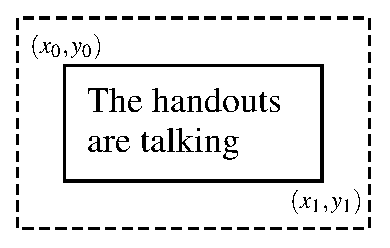
\includegraphics[width=\textwidth]{elem-bbox.eps}
        \caption{A \texttt{BBox} object}
        \label{fig:elem-bbox}
    \end{subfigure}%
    ~ 
    \begin{subfigure}[t]{0.48\textwidth}
        \centering
        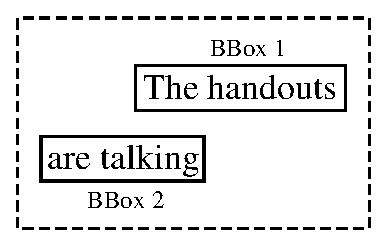
\includegraphics[width=\textwidth]{elem-bboxgroup.eps}
        \caption{A \texttt{BBoxGroup} object}
        \label{fig:elem-bboxgroup}
    \end{subfigure}
    \caption{Examples of \texttt{BBox} and \texttt{BBoxGroup} objects}
\end{figure}

\subsection{The BBoxGroup class}

A \texttt{BBoxGroup} object is simply a collection of \texttt{BBox} objects. Usually the \texttt{BBox} objects contained in a \texttt{BBoxGroup} object are closely related to each other, for example a sentence across multiple lines can be expressed as a \texttt{BBoxGroup} object. \Cref{fig:elem-bboxgroup} shows an example \texttt{BBoxGroup} object.

The \texttt{BBoxGroup} class defines the atomic level of alignment input at the OCR side. The single mapping from a \texttt{BBoxGroup} object to the corresponding parts of the audio file cannot be further divided.

\subsection{The BBoxGroups class}

As the class name suggests, a \texttt{BBoxGroups} object is simply a collection of \texttt{BBoxGroup} objects. In the actual implementation, the \texttt{BBoxGroups} class inherits from the Python's built-in \texttt{list} class, and hence a \texttt{BBoxGroups} object has all the properties of Python lists.

The output of the OCR engine is a \texttt{BBoxGroups} object, which is a list of atomic objects for the alignment process. 

\section{Elements Related to the Speech Recogniser}

\subsection{The TStamp class}

A \texttt{TStamp} object represents a timestamp in the audio file. The class defines three attributes: \texttt{min} (minutes), \texttt{sec} (seconds, within range [0, 59]) and \texttt{msec} (milliseconds, within range [0, 999]).

\subsection{The TInterval class}

A \texttt{TInterval} object represents an interval in the audio file which consists of two \texttt{TStamp} objects, indicating the starting timestamp and the ending timestamp respectively. This class provides an straightforward way of representing segments of the audio file.

\subsection{The WStamp class}

The class name \texttt{WStamp} stands for `word with a timestamp'. A \texttt{WStamp} object represents a recognised word and the associated starting timestamp as in the input audio file. This class forms the basis of the speech recogniser output, which is also called the transcript of the audio file. 

\subsection{The WStamps class}

A \texttt{WStamps} object is a collection of multiple \texttt{WStamp} objects. Similar to the \texttt{BBoxGroups} class, the \texttt{WStamps} class also inherits from the Python built-in \texttt{list} class.

This class can be used to describe the speech recogniser output (also called the `transcript'). In the actual system implementation, the output of the speech recogniser is just a \texttt{WStamps} object.

\section{Elements Related to the Alignment Algorithm}

\subsection{The TIntervalGroup class}

A \texttt{TIntervalGroup} object is a collection of multiple \texttt{TInterval} objects. In the final alignment result, each \texttt{BBoxGroup} object uniquely matches a \texttt{TIntervalGroup} object. Hence, the \texttt{TIntervalGroup} class is a fundamental part of the alignment result.

\subsection{The Match class}

A \texttt{Match} object simply represents a single match in the alignment result, which consists of a {BBoxGroup} object and a \texttt{TIntervalGroup} object. 

\subsection{The Matches class}
\label{sec:basic-elem-matches}

A \texttt{Matches} object is a collection of multiple \texttt{Match} objects. This class also inherits from the Python built-in \texttt{list} class. In the actual implementation, the final alignment result is a \texttt{Matches} object. \Cref{fig:elem-matches} shows the relationships between different classes, starting from a \texttt{Matches} object.

\begin{figure}[t]
    \centering
    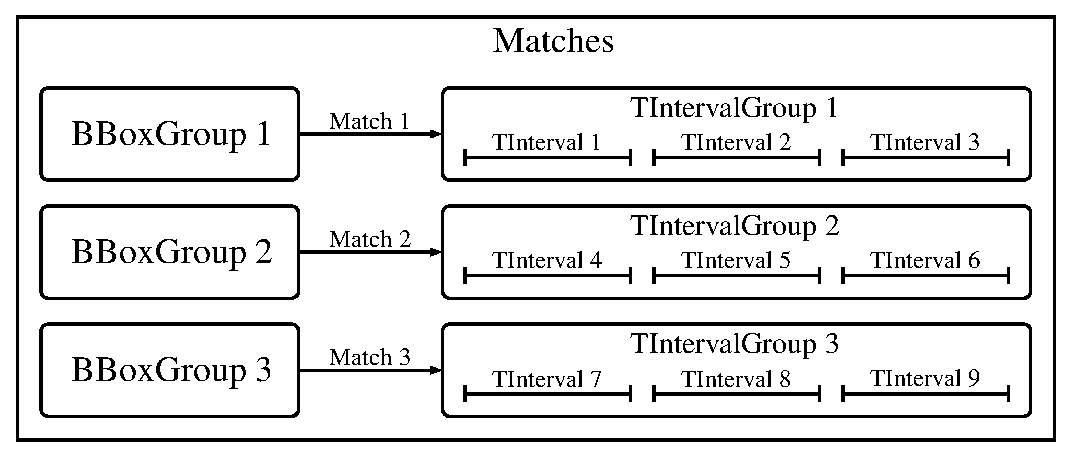
\includegraphics[width=0.9\textwidth]{elem-matches.eps}
    \caption{Relationships between different classes inside a \texttt{Matches} object}
    \label{fig:elem-matches}
\end{figure}

\section{System Architecture Revisited}

We shall now revisit the system architecture based on the knowledge of the basic element definitions. \Cref{fig:elem-sys-diagram} shows the updated diagram labelled with the defined classes of the basic elements.

\begin{figure}[!hb]
    \centering
    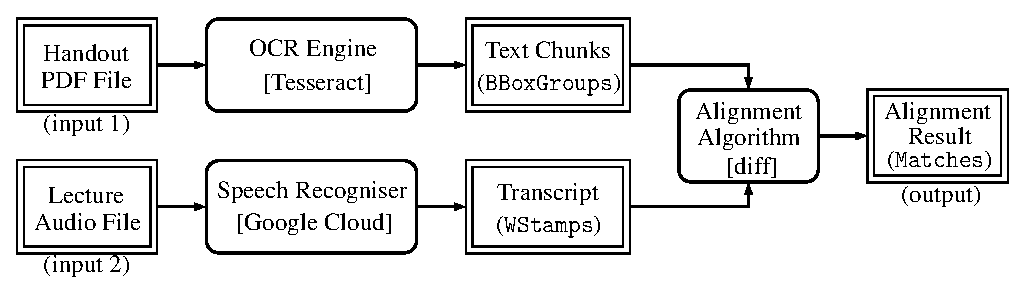
\includegraphics[width=0.95\textwidth]{elem-sys-diagram.eps}
    \caption{Basic elements as inputs / outputs within the system}
    \label{fig:elem-sys-diagram}
\end{figure}